\documentclass[12pt]{article}
 \usepackage[margin=1in]{geometry}
\usepackage{amsmath,amsthm,amssymb,amsfonts}
\usepackage{bm}
\usepackage{graphicx}

\newcommand{\N}{\mathbb{N}}
\newcommand{\Z}{\mathbb{Z}}

\newenvironment{solution}[2][Solution]{\begin{trivlist}
\item[\hskip \labelsep {\bfseries #1}\hskip \labelsep {\bfseries #2.}]}{\end{trivlist}}
%If you want to title your bold things something different just make another thing exactly like this but replace "solution" with the name of the thing you want, like theorem or lemma or whatever

\begin{document}


\title{Homework 4}
\author{Due Date: May 2, 2018}
\date{}

\maketitle

\begin{solution}{1}
1) The VC dimension of $H$ is 3. The $H$ is able to shatter 3 points with any label assigments in one dimension. But it fails when there are 4 points with the specified labels shown in below. \\
\begin{center}
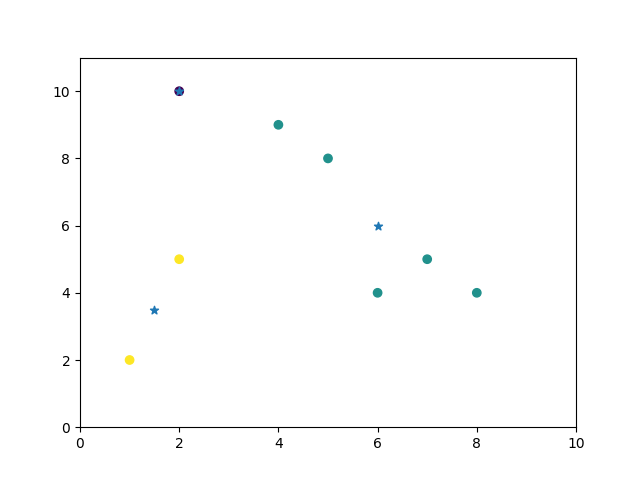
\includegraphics[angle = 0, width = .4\textwidth]{./images/fig6.png}
\end{center}

2) After rearangement of this formula, we obtain
$$
	\frac{13}{\epsilon} 2^{8VC(H)-\epsilon m-3} \leq \delta
$$
It means that t a hypothesis consistent with m examples will have error at least $\epsilon$ with probability $\frac{13}{\epsilon} 2^{8VC(H)-\epsilon m-3}$.

\end{solution}

\begin{solution}{2}
The VC dimension is 3. The concept $f$ can not seperate the 4 points shown below while it shatters all 3 data points.\\
\begin{center}
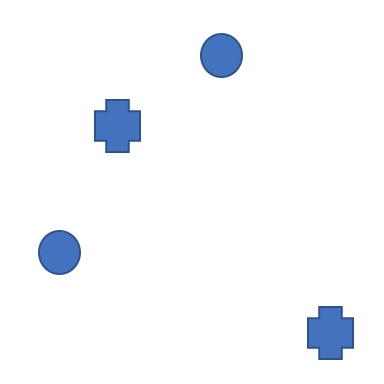
\includegraphics[angle = 0, width = .4\textwidth]{./images/fig4.png}
\end{center}
\end{solution}

\begin{solution}{3}
1) By regularizing $w_2$, feature $x_2$ vanishes. The seperator achieves the lowest error when it is located near blue line. The training error increases. 3 points are misclassified.\\
2) By regularizing $w_1$, feature $x_1$ vanishes. The seperator achieves the lowest error when it is located near red line. The training error stay the same(zero).\\
3) By regularizing $w_0$, bias vanishes. The seperator achieves the lowest error when it is located near yellow line. The training error stay the same(zero).
\begin{center}
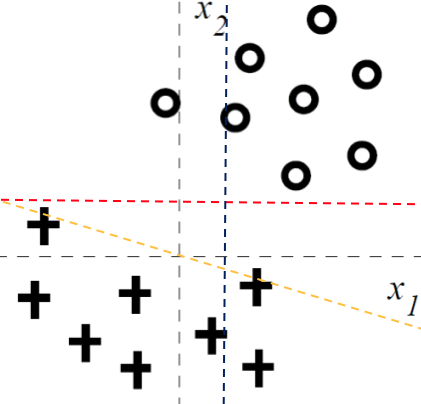
\includegraphics[angle = 0, width = .4\textwidth]{./images/fig5.png}
\end{center}
\end{solution}

\begin{solution}{4}
1) First $w_1$ will become 0, then $w_2$, Because $w_1$ contributes little to classify the data points correctly.\\
2) Since the seperator tries to minimize the misclassified error, $w_0$ will take the value near the red line.\\
3) $w_0$ may move upwards a little if there are more '+' classes. The sepearator will have a high bias to predict '+' class.
\end{solution}

\end{document}